\subsubsection{UART}
\begin{itemize}
	\itemsep-.5em
	\item Handshaking Lines
	\begin{itemize}
		\itemsep-.5em 
		\item \textbf{DSR} Data Set Ready
		\item \textbf{DTR} Data Terminal Ready
		\item \textbf{RTS} Request to Send
		\item \textbf{CTS} Clear to Send
	\end{itemize}
	\item Communication Lines
	\begin{itemize}
		\itemsep-.5em
		\item \textbf{TxD} Transmitted Data
		\item \textbf{RxD} Received Data
	\end{itemize}
\end{itemize}

\subsubsection{RS-232 \refskript{9.3.8}}
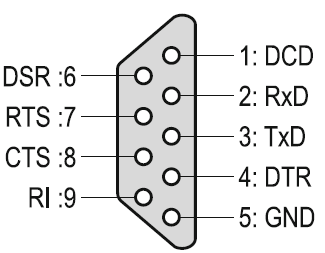
\includegraphics[width=.4\columnwidth]{"Images/RS232Connector.png"}
Point to point connection.
The transfer-speed is highly dependent on the transmission line length.

\subsubsection{RS-422}
Bus connection with a maximum of 10 receivers (more with repeaters or buffers).

\subsection{Ring Buffer}
A ring buffers works with the FIFO principle.